%==================================================================%
% Author : Perez Ruiz, Alejandro                                   %
% Version: 1.0, 26/05/2011                                         %                                                                                     % Manual de instalaci�n/desinstalaci�n                             %
%==================================================================%
\documentclass[a4paper,11pt]{article}

\usepackage[latin1]{inputenc}
\usepackage{url}
\usepackage{amsfonts}
\usepackage[spanish,activeacute]{babel}
\usepackage{graphicx}
\usepackage{url}

\title{Manual de Usuario para la instalaci�n y desinstalaci�n}

\author{Alejandro P�rez \\ Dpto. Matem�ticas, Estad�stica y Computaci�n \\
		Universidad de Cantabria (Santander, Espa�a)}

\begin{document}

\maketitle
\section{Instalaci�n y desinstalaci�n}
Los dos plugins presentados en este proyecto est�n embebidos en Microsoft Visual Studio 2010 Professional, por lo tanto, el primer paso es obtener este IDE e instalarlo en el computador.

\subsection{Instalaci�n del plugin destinado a la creaci�n de modelos}
El plugin destinado a crear modelos espec�ficos del hogar inteligente debe ser el primero en ser instalado, para ello:
\begin{enumerate}
\item Acudimos a la siguiente direcci�n web:

    {\url{http://www.alumnos.unican.es/apr85/download.html}}
    
     y descargamos el plugin denominado \emph{SmartHomeModeller.msi}.
\item Vamos al lugar donde hemos descargado el archivo anterior y hacemos doble click sobre �l.
\item Seguimos los pasos que nos aparecen en el asistente para finalizar la instalaci�n, teniendo en cuenta el paso en el que se ofrece la posibilidad de elegir la ubicaci�n para la instalaci�n.\\\\
    \begin{center}
            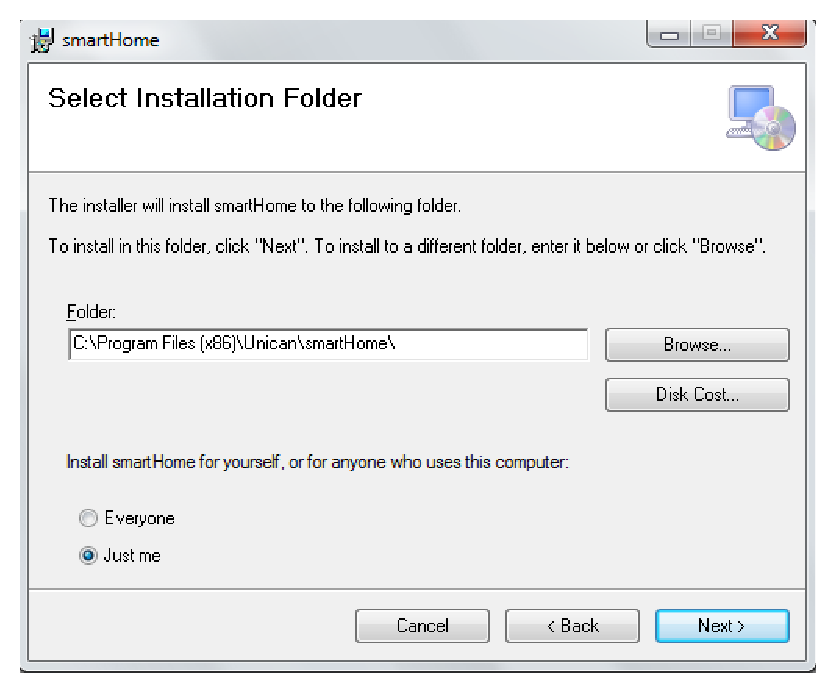
\includegraphics[width=.65\linewidth]{images/ubicacionModeller.eps}
            \vspace{1cm}
     \end{center}

\end{enumerate}

\subsection{Desinstalaci�n del plugin destinado a la creaci�n de modelos}
Existen dos formas de desinstalar el plugin:
\begin{enumerate}
\item Acudiendo en nuestra versi�n de Windows a \emph{Panel de Control}, seguidamente buscamos la opci�n de desinstalar programas, para luego encontra nuestro plugin a trav�s de su nombre, \emph{SmartHome}.
\item Si poseemos el archivo de instalaci�n (\emph{SmartHomeModeller.msi}), abri�ndolo nos aparecer� la opci�n de desinstalar (\emph{Remove smartHome}).
     \begin{center}
            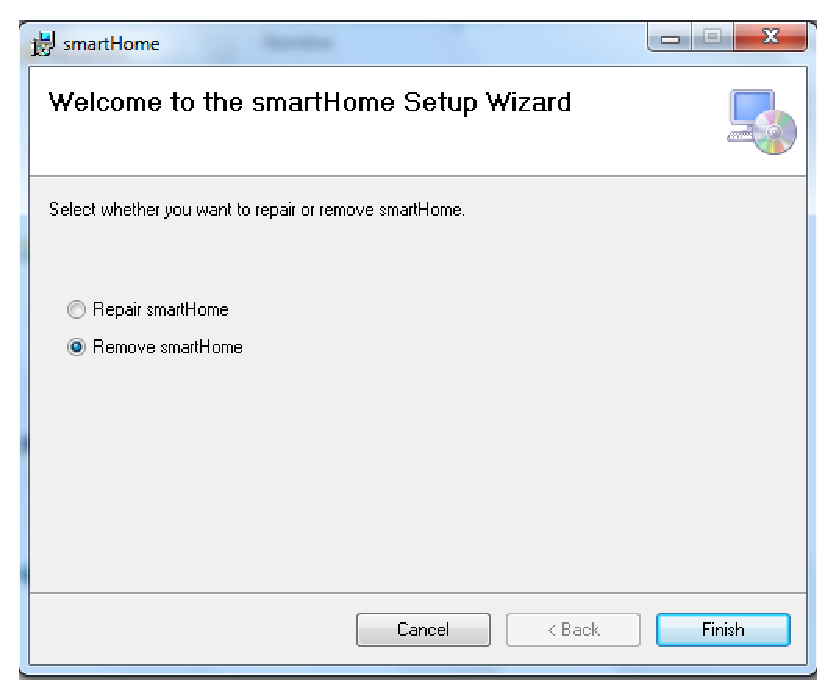
\includegraphics[width=.65\linewidth]{images/removeModeller.eps}
            \vspace{1cm}
     \end{center}
\end{enumerate}

\subsection{Instalaci�n del plugin que permite la creaci�n de configuraciones}
 Este plugin debe ser instalado en segundo lugar, puesto que necesita del anterior para permitirnos crear modelos de un hogar inteligente y/o autom�tico. Para realizar la instalaci�n se debe proceder a seguir los siguientes pasos:
 \begin{enumerate}
 \item Acudimos a la siguiente direcci�n web: 
    
    {\url{http://www.alumnos.unican.es/apr85/download}}
     
     y descargamos el plugin denominado \emph{smartHomeProject.vsix}.
 \item Vamos al lugar donde hemos descargado el archivo anterior y hacemos doble click sobre �l.
 \item Seguimos el asistente de instalaci�n para finalizar.

 \end{enumerate}

 \subsection{Desinstalaci�n del plugin que permite la creaci�n de configuraciones}
 Para desinstalar este plugin debemos abrir Visual Studio 2010 y realizar los siguientes pasos:
 \begin{enumerate}
 \item Ve a \emph{Tools} y selecciona \emph{Extension Manager}.
    \begin{center}
            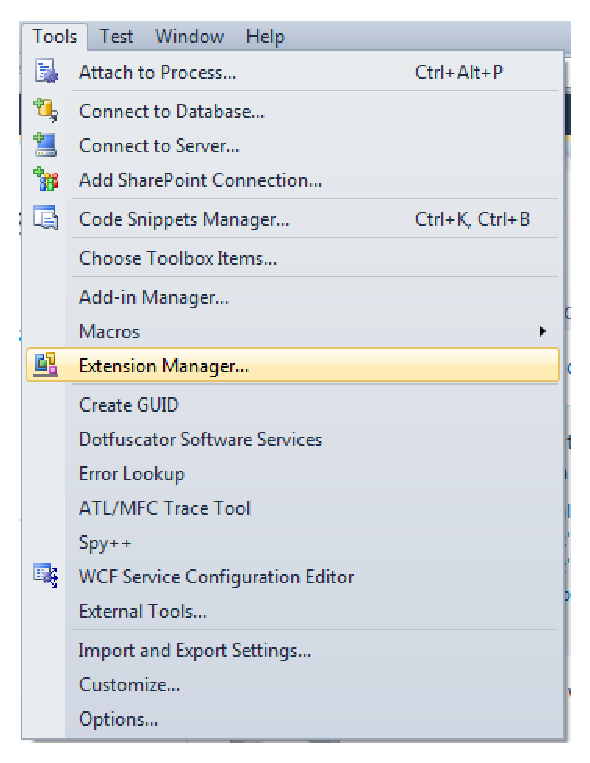
\includegraphics[width=.65\linewidth]{images/removeProject.eps}
            \vspace{1cm}
     \end{center}
 \item Selecciona la extensi�n denominada \emph{Smart Home Project} y pulsamos \emph{Uninstall}.

 \end{enumerate}

 \section{Actualizaciones}
 Si en la p�gina web \url{http://www.alumnos.unican.es/apr85} aparece una nueva versi�n de alguno de los plugins que tenemos instalados, y queremos actualizar, es necesario desinstalar los actuales que se tienen en el ordenador siguiendo los pasos descritos anteriormente, para volver a descargar e instalar las nuevas versiones.


\end{document} 